\section{Simulation Analysis}
\label{sec:simulation}

\paragraph{}
In this section, we can find the results of each topic required in the simulation analysis. The numeric results or graphics are presented alongside a short explanation of the interpretation of the problem. All of the results were obatined usig NGSpice and the section is divided in two different subsections. 

In this part of the lab, we tried to build the circuit in such a way that it would be as similar as possible as the one used in the Octave theoretical part. The most important difference between both approaches is that in Ngspice we had to use more diodes in the regulator circuit than in Octave. This is because while in Octave we used the standard diode voltage ($0.7 V$), requiring 17 diodes, in Ngspice that wasn't possible because diodes have varying voltages. Given that, our Ngspice voltage regulator circuit is made of 23 diodes.

Another difference from the Octave model, is that the ideal diode model used in the envelope circuit is not possible to replicate in Ngspice. However, this does not affect the final results because the transformer conversion factor was updated to compensate the fact that there is going to be a voltage drop in the envelope circuit diodes.

\subsection{Envelope Circuit Output}

\begin{figure}[H] \centering
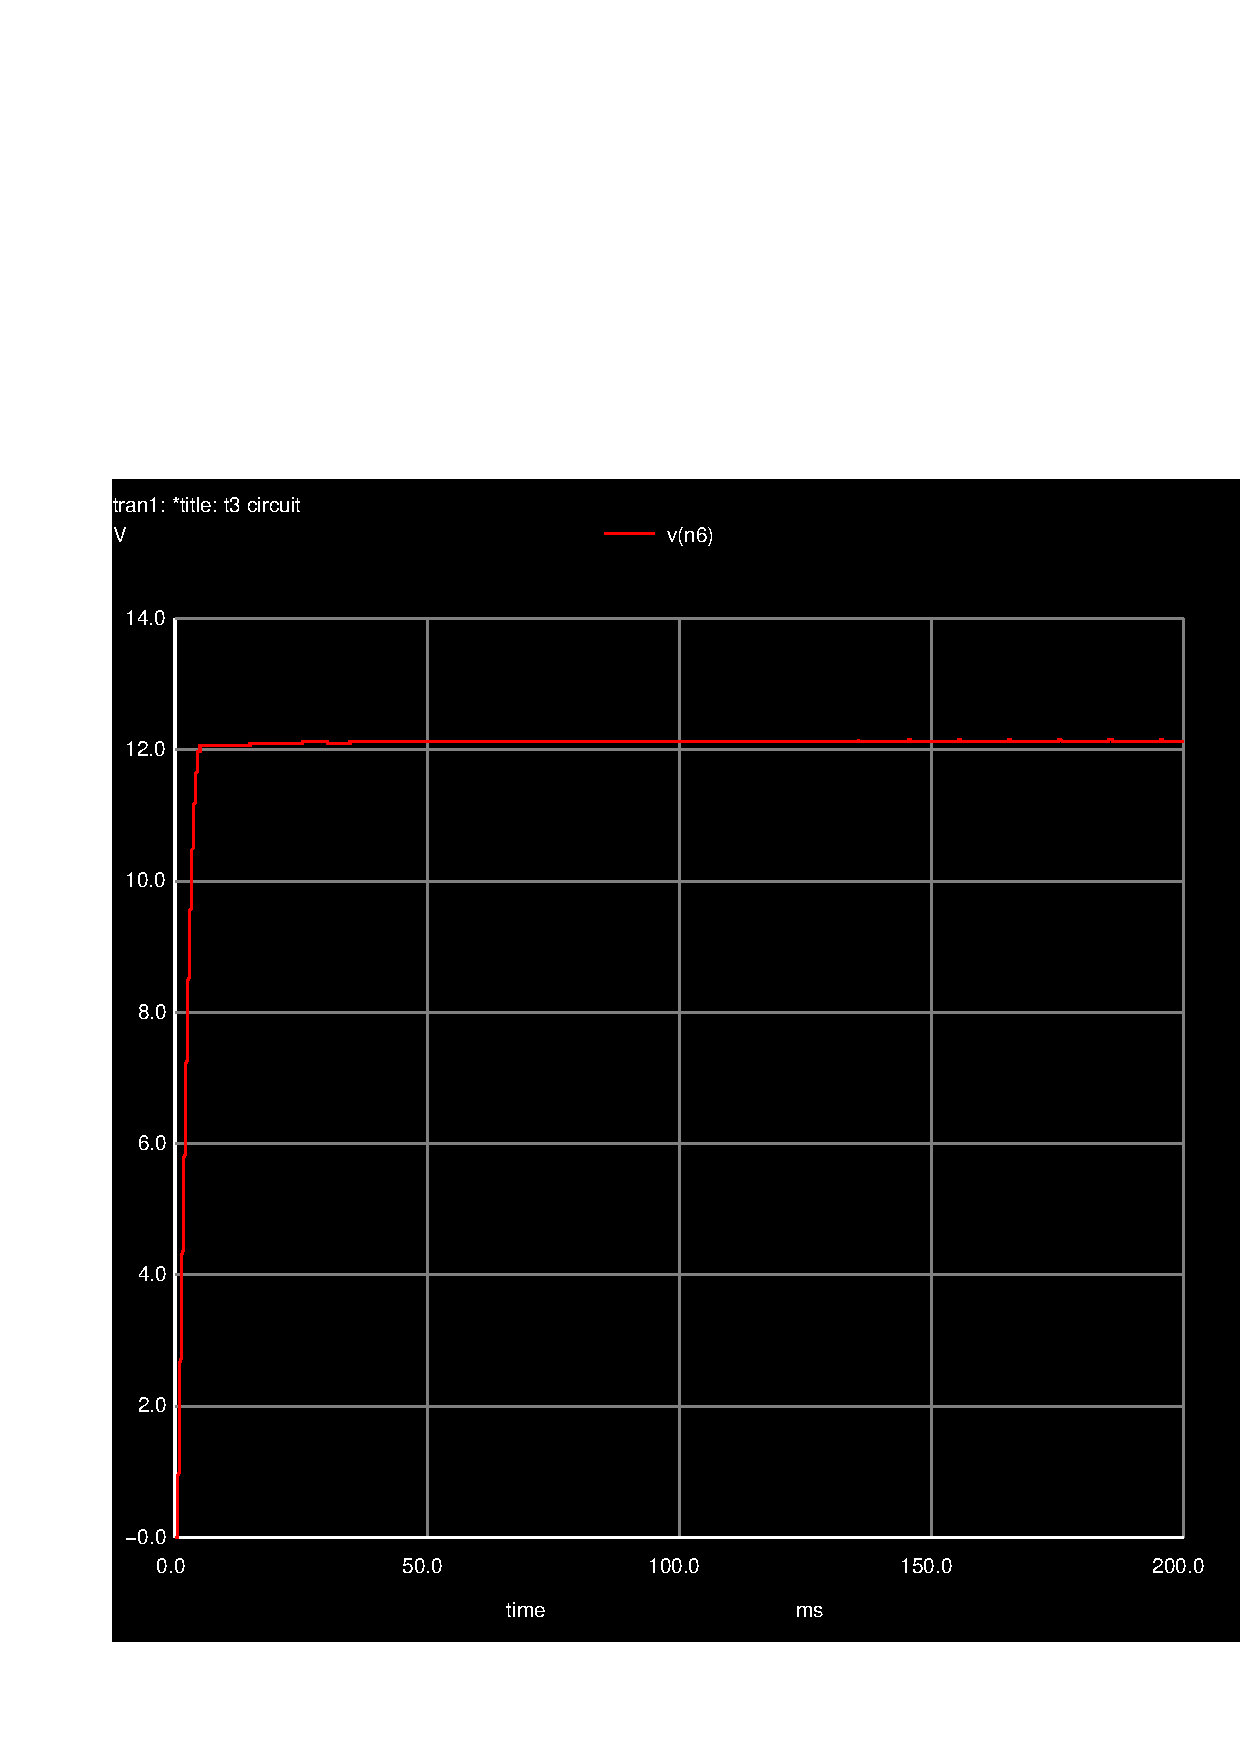
\includegraphics[trim= 0cm 0cm 0cm 10cm, clip, width=0.7\textwidth]{trans1.pdf}
\caption{The final envelope detector circuit voltage $v_0$ during 10 periods}
\label{fig:sim_envelope}
\end{figure}

\paragraph{}
In the graphic above, it is possible to see that, even though it is not the final result of the whole converter, it is already very close to $12V$. It is important to note that, if we zoom in, there will be a certain level of ripple that may affect our desired result, given that the signal hasn't gone throught the voltage regulator yet. Still on this topic, a particularity of Ngspice is the rising line at the very beginning which clearly stands for some transient the software uses.

\subsection{Circuit Output}

\paragraph{}
In this part the total output of the circuit is analysed.

\begin{figure}[H]\centering
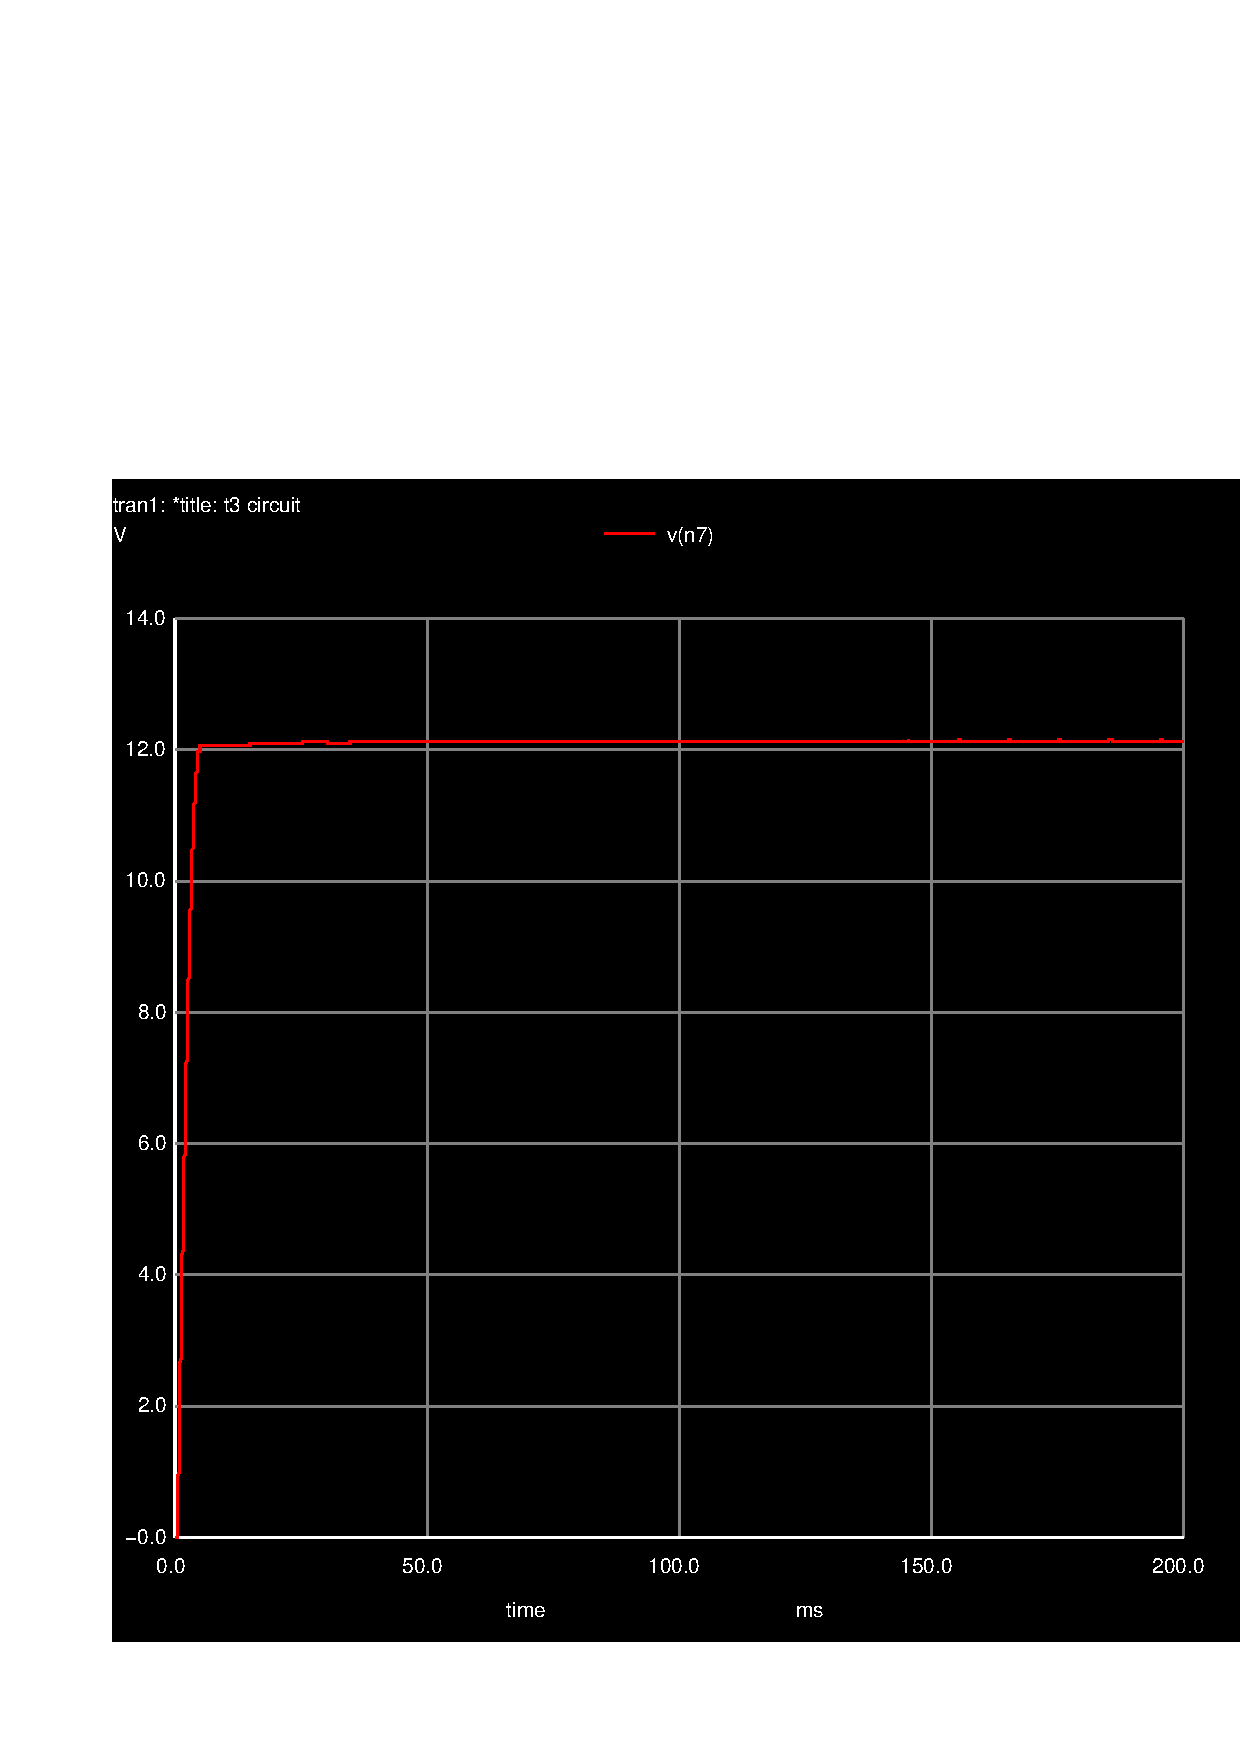
\includegraphics[trim= 0cm 0cm 0cm 10cm, clip, width=0.7\textwidth]{trans2.pdf}
\caption{The final output voltage $v_0$ during 10 periods}
\label{fig:sim_output}
\end{figure}

In the graphic above, the output voltage is represented. Looking at it is enough to understand that the final voltage is very close to the desired $12V$, however the difference that remains will be discussed below.

\begin{figure}[H]\centering
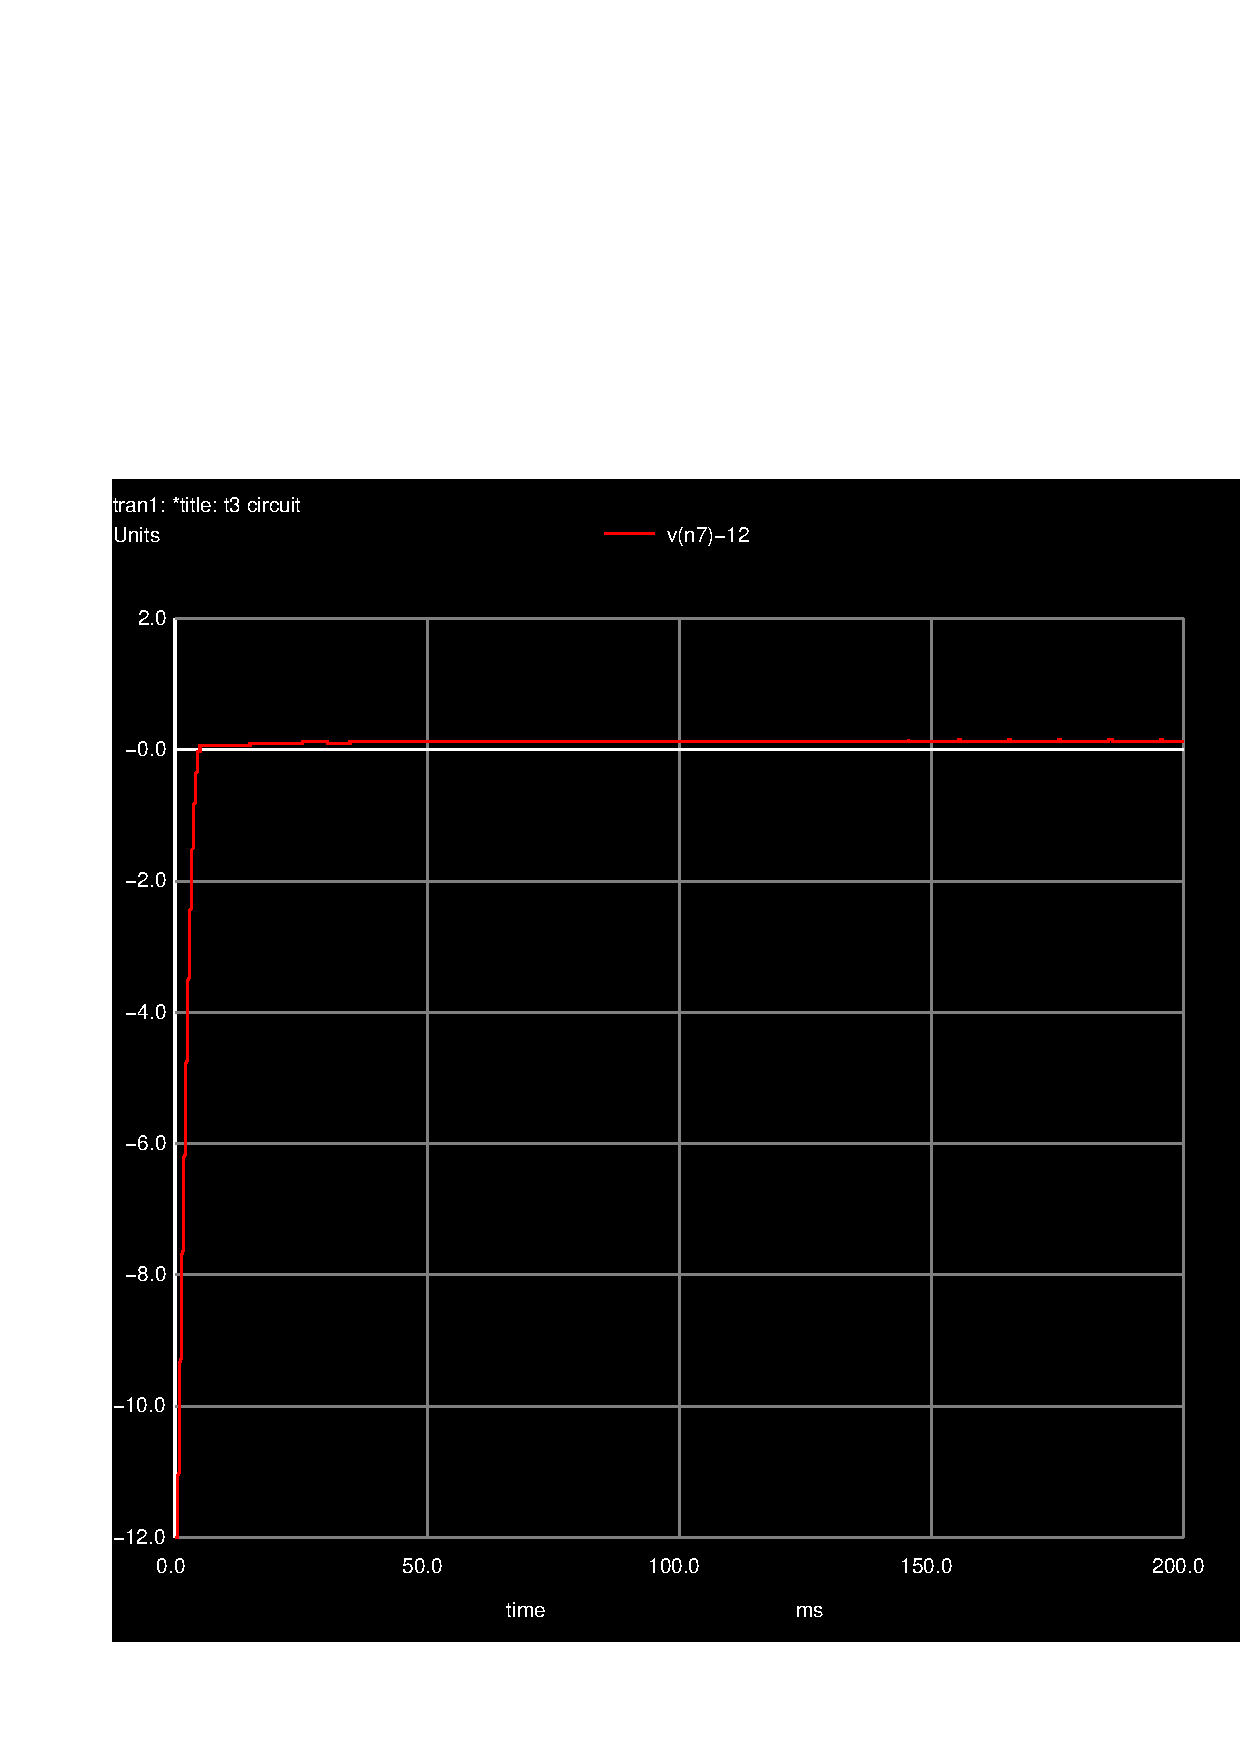
\includegraphics[trim= 0cm 0cm 0cm 10cm, clip, width=0.7\textwidth]{trans3.pdf}
\caption{The final output voltage $v_0$ subtracted by 12 during 10 periods}
\label{fig:sim_outputdiff}
\end{figure}

The graphic above essentialy shows the ripple of the circuit, which is basically how much the output voltage deviates from $12V$ and, once again, the results are pretty satisfying, with the line being very close to zero for most of the 10 periods. Still, below we can find a table with more accurate ripple data at a numerical level, which will confirm the theory that the simulation was well-succeeded.


\begin{table}[H] \centering
  \begin{tabular}{|l|r|}
    \hline    
    {\bf Data} & {\bf Value} \\ \hline
    \input{op_TAB}
  \end{tabular}
  \caption{}
 \label{tab:op}
\end{table}

From the table above, we can see that the average has a pretty good result being pratically $12V$. When it comes to the ripple, it also has a very good result, with an order of significance in the hundredths.
